\section{Einleitung}
Laut IEEE kann das requirements engineering unterteilt werden in:
\begin{itemize}
	\item Anforderungserhebung (requirements elicitation),
	\item Anforderungsanalyse (requirements analysis),
	\item Anforderungsspezifikation (requirements specification) und
	\item Anforderungsbewertung (requirements validation)
\end{itemize}
Diese Tätigkeiten überlappen einander und werden oft auch mehrfach – iterativ – durchgeführt. (Wikipedia)\\
\\
Requirements sind nicht gegeben, sondern müssen erarbeitet werden und im Laufe des Entwicklungsprozess verfeinert und verbessert werden.
Interdisziplinäre Disziplin mit Menschenkontakt. Abbildung der informalen Welt der Stakeholder auf die formale Welt der Entwickler/Verhalten der Software.\\
In RE muss der Analyst verstehen:
\begin{itemize}
	\item System-as-is
	\item System-to-be
	\item System-to-be-next
\end{itemize}
Daraufhin wird ein Model der aktuellen Situation erstellt und das in ein Model der vorgestellten Situation überführt. (Grob zsmf)
\subsection{non-functional R}
\begin{itemize}
	\item Bedingungen die an das System als Ganzes gestellt werden, z.B. Zeitbeschränkungen, Performance, Standards, den Entwicklungsprozess
	\item \textbf{Aufteilung in}
	\begin{itemize}
		\item \textit{Product} Effizienz (Performance, Speicherbedarf), Usability, Zuverlässigkeit
		\item \textit{Organisational} Standards, Entwicklungsprozess
		\item \textit{External} Ethische, Gesetzliche, Interoperabilität
	\end{itemize}
	\item oftmals kritischer als functional, da User bei Fehlverhalten eines Dienstes (=functional R) einen Weg drum herum findet. Bei fehlerhafter NFR ist dies nicht so leicht möglich.
	\item quantisierbar spezifizieren um objektiv testen zu können. Dazu folgende Kriterien
	\begin{table}[!h]
		\begin{tabular}{|l|l|}
			\hline
			\textbf{Eigenschaft}	& \textbf{Messeinheit}\\
			\hline
			Speed		& Operationen/Sekunde; Reaktionszeit auf Usereingabe\\
			Ease of Use	& Einarbeitungszeit; Hilfsfenster\\
			Zuverlässigkeit & Durchschnittszeit bis Fehler eintritt\\
			Robustheit & Was passiert mit Daten nach Fehler?\\
			& Wie schnell lässt sich das System nach Fehler neustarten?\\
			\hline
		\end{tabular}
	\end{table}
	
\end{itemize}

\subsection{functional R}
\begin{itemize}
	\item Aussagen über Dienste die das System liefern muss, speziell konkrete Features, wie reagiert das System auf Eingaben, bei bestimmten Situationen.
	\item Manchmal Aussage darüber was das System in Situation grade \textit{nicht} machen soll.
	\item \textbf{Aspekte:}
	\item \textit{Data:} Struktur, Verwaltung, Zugriff, Übertragung
	\item \textit{Functions:} Input, Output, Verarbeitung
	\item \textit{Verhalten:} beobachtbares Verhalten des Systems (auch in Fehlersituationen)
\end{itemize}


\subsection{Domain Requirements}
Ergeben sich aus der Anwendungsdomäne des Systems und spiegeln die Charakteristik und Bedingungen der Domäne wieder. Kann sowohl non-functional als auch functional R sein.

\begin{figure}[!h]
	\centering
	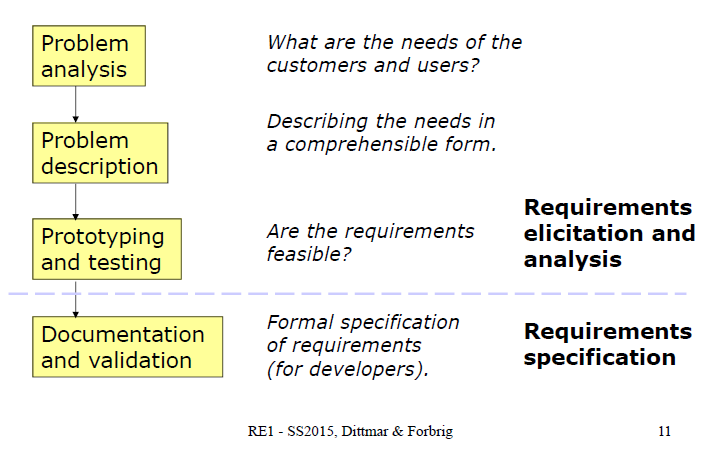
\includegraphics[scale=0.5]{img/define_req.png}
\end{figure}

\subsection{Requirements Specification (RS)}
\textbf{Product Constraints} bestimmen
\begin{enumerate}
	\item Zweck des Produkts\\
	Aufgabe, Ziel, Was soll das Produkt bringen? Wichtige Punkte
	\begin{itemize}
		\item Welchen Vorteil liefert das Produkt?
		\item Ist der Vorteil messbar?
		\item Ist der Aufwand für den Vorteil rechtfertigbar?
	\end{itemize}
	\item Client, Kunde, Stakeholder
	\item Nutzer des Produkts
	\item Requirements Bedingungen
	\item Definitionen, Nomenklatur
	\item relevante Fakten
	\item Annahmen
\end{enumerate}
\textbf{Functional Req.} bestimmen
\begin{itemize}
	\item Scope des Produkts\\
	The features and functions that characterize a product, service, or result.
	\item Functional and Data Req\\
	Spezi der Dienste und Datenstruktur
\end{itemize}
\textbf{Non-Functional Req.} bestimmen

\subsection{Software Requirements Specification (SRS)}
Spezifikation für ein Softwareprodukt.\\
Eigenschaften einer guten SRS:
\begin{itemize}
	\item Korrekt, Komplett, Konsistent, Verifizierbar...
	\item eindeutig -> jede spezifizierte Anforderung hat genau eine Interpretation
	\item Grundlagen, die eine SRS betrachten/beantworten sollte
	\begin{itemize}
		\item Functionality: Was soll die Software leisten?
		\item External Interfaces: Interaction with people
		\item Performance: Geschwindigkeit, Verfügbarkeit, ...
		\item Attributes: Portabilität, Korrektheit, Wartbarkeit, Sicherheit...
		\item Design Contraints for the impl:
	\end{itemize}
\end{itemize}

\subsection{Main Activities in RE}
\begin{itemize}
	\item Erhebung der R. (informal)\\
	Welche Probleme bewältigen? Wer ist Kunde, Stakeholder, Nutzer? Techniken: Interviews, Brainstorming, Prototyping
	\item Model and Analysing der R -> Ergebnis: Formale R
	\item Kommunikation der R\\
	Formale R müssen auch für Stakeholder verständlich sein
	\item Abgleich/Verifikation der formalen R mit Vorstellungen der Stakeholder
	\item Weiterentwicklung der R \\
	Vorstellung des Softwaresystems kann Stakeholder/Nutzer/Kunde dazu veranlassen R umzuformulieren
\end{itemize}